\section{Introduction}

\begin{frame}{Introduction}
  \begin{block}{Introductory problem : POWER SUPPLY problem}
  Let $C$ be a set of customer with fixed demands, $P$ be a set of power stations with fixed capacity and $G = (V,E)$ be a bipartite graph where $V = \{C \cup P$\} with weights on the vertices.  \hfill \break
  \pause
  \hfill \break
  Can $G$ be partitioned into subtrees, such that each subtree contains exactly one power supply $P$ s.t the sum of the demands of the $C$ vertices (customers) in each subtree is no more than the capacity of the $P$ vertex (power station) in it?

  \end{block}
\end{frame}

\begin{frame}{Introduction}
\begin{columns}
    \begin{column}{0.5\textwidth}
        \begin{figure}
        \centering
        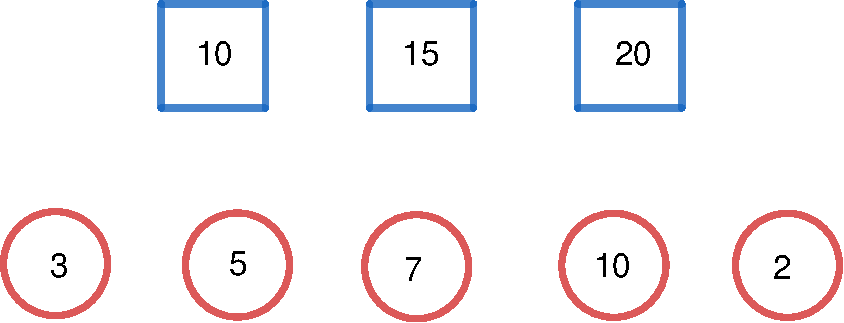
\includegraphics[width=0.9\textwidth]{img/ps1.pdf}
        \caption{Input graph $G$ where the blue vertices are the power stations and red vertices are the customers.}
        \label{fig:ps}
        \end{figure}
    \end{column}
    \pause
    \begin{column}{0.5\textwidth}
        \begin{figure}
        \centering
        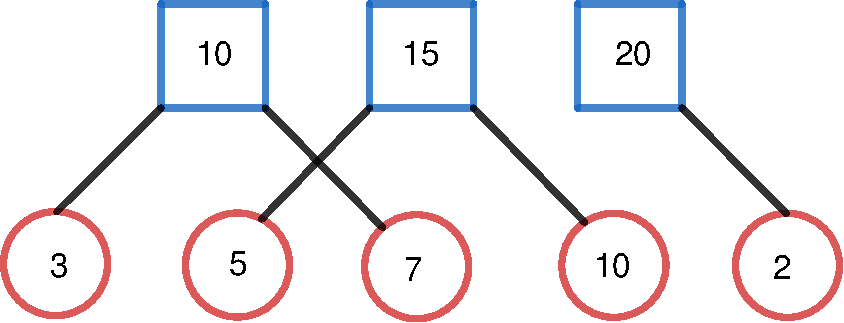
\includegraphics[width=0.9\textwidth]{img/ps2.pdf}
        \caption{A feasible solution to the POWER SUPPLY problem.\hfill \break}
        \label{fig:circle}
        \end{figure}
    \end{column}
\end{columns}

\begin{block}{Theorem (Ito et al.)}
The POWER SUPPLY problem is NP-complete \cite{DBLP:journals/tcs/ItoDHPSUU11}.
\end{block}
\end{frame}

\subsection{Power Supply Reconfiguration problem}
\begin{frame}{POWER SUPPLY RECONFIGURATION problem}
Suppose now that we are given two feasible solutions $s_0$ and $s_t$ of the POWER SUPPLY problem and are asked: \hfill \break 

Can one solution be transformed into the other by moving only one customer at a time and always remaining feasible?
\pause
\begin{columns}
    \begin{column}{0.5\textwidth}
        \begin{figure}
        \centering
        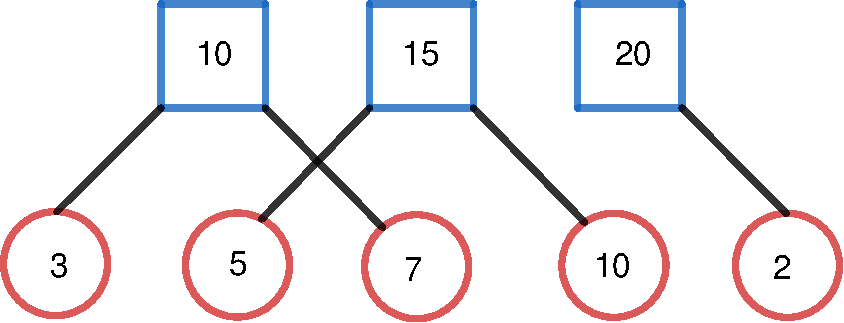
\includegraphics[width=0.9\textwidth]{img/ps2.pdf}
        \caption{Feasible solution $s_0$.}
        \label{fig:circle}
        \end{figure}
    \end{column}
    \begin{column}{0.5\textwidth}
        \begin{figure}
        \centering
        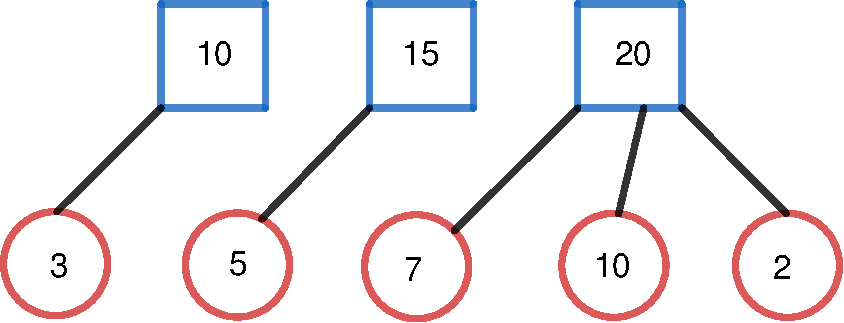
\includegraphics[width=0.9\textwidth]{img/ps4.pdf}
        \caption{Feasible solution $s_t$.}
        \label{fig:circle}
        \end{figure}
    \end{column}
\end{columns}
\end{frame}

\begin{frame}{POWER SUPPLY RECONFIGURATION problem}
\begin{columns}
    \begin{column}{0.3\textwidth}
        \begin{figure}
        \centering
        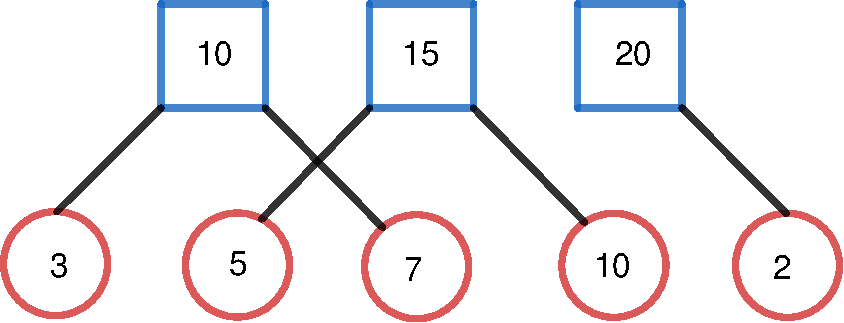
\includegraphics[width=1.1\textwidth]{img/ps2.pdf}
        \caption{Feasible solution $s_0$.\hfill \break \hfill \break \hfill \break \hfill \break}
        \label{fig:circle}
        \end{figure}
    \end{column}
    \begin{column}{0.3\textwidth}
        \begin{figure}
        \centering
        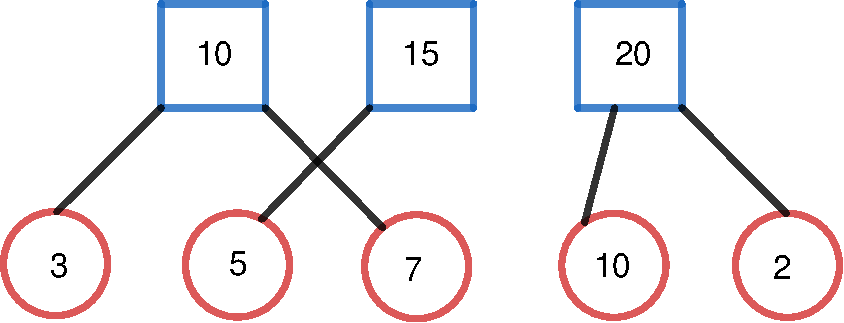
\includegraphics[width=1.1\textwidth]{img/ps3.pdf}
        \caption{Intermediate feasible solution $s_i$ where customer $10$ is moved.\hfill \break \hfill \break}
        \label{fig:circle}
        \end{figure}
    \end{column}
    \begin{column}{0.3\textwidth}
        \begin{figure}
        \centering
        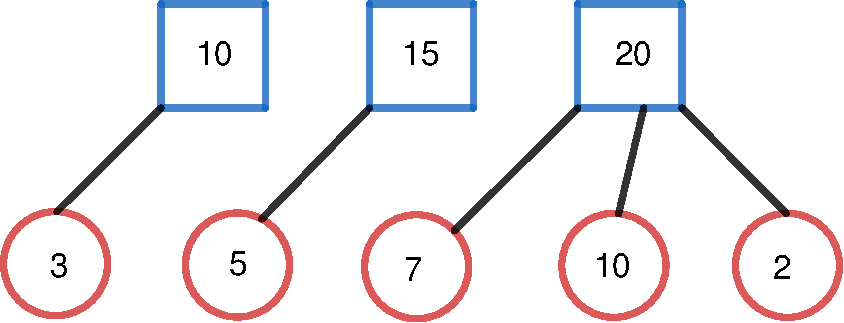
\includegraphics[width=1.1\textwidth]{img/ps4.pdf}
        \caption{Target feasible solution $s_t$ where customer $7$ is moved from previous intermediate solution.\hfill \break}
        \label{fig:circle}
        \end{figure}
    \end{column}
\end{columns}

    \begin{block}{Theorem (Ito et al.)}
    POWER SUPPLY RECONFIGURATION problem is PSPACE-complete \cite{DBLP:journals/tcs/ItoDHPSUU11}.
    \end{block}
\end{frame}

\section{Reconfiguration problems}
\subsection{Definition}
\begin{frame}{RECONFIGURATION problems}
  \begin{block}{Definition}
    Reconfiguration problems are computational problems in which we wish to find a step-by-step transformation between two feasible solutions of a problem such that all intermediate results are also feasible.
  \end{block}
\end{frame}


\begin{frame}{RECONFIGURATION problems}
    \begin{block}{Graph-theoric perspective}
    \begin{itemize}
        \item Reconfiguration graph where : 
        \begin{enumerate}
            \item The vertex set consists of all possible configurations (solutions).
            \item Two nodes are connected if the corresponding configurations can each be obtained from the other by the application of a single transformation rule, a \textit{reconfiguration step}.
        \end{enumerate}
        \item Any path or walk in the Reconfiguration graph $=$ \textit{Reconfiguration sequence}. 
    \end{itemize}
  \end{block}
\end{frame}

\section{Main themes}
\begin{frame}{RECONFIGURATION problems}
    \begin{block}{Main themes}
        \begin{enumerate}
            \item SATISFIABILITY RECONFIGURATION problems.
            \item SLIDING TOKENS problems. 
            \item SUBSET SUM RECONFIGURATION problems.
        \end{enumerate}
    \end{block}
\end{frame}



